\documentclass[journal]{IEEEtran}
%\documentclass[conference]{IEEEtran}
\hyphenation{op-tical net-works semi-conduc-tor}
\usepackage{graphicx}
\graphicspath{{./images/}}

\begin{document}
\title{3D Indoor Mapping Using ROS and Microsoft Kinect Sensor}
\author{Chirag~Shah
        and~Srijal~Poojari}% <-this % stops a space
\markboth{Journal of \LaTeX\ Class Files,~Vol.~14, No.~8, August~2015}%
{Shell \MakeLowercase{\textit{et al.}}: Bare Demo of IEEEtran.cls for IEEE Journals}

\maketitle
\begin{abstract}
The objective of this project is to create a 3D map of a given environment using a depth camera (Microsoft Kinect) and send this information over a Wi-Fi network to a laptop. This will enable mounting of the camera on a robot/quadcopter and create 3D  map of an indoor environment.

We used the ROS framework running on a laptop and a Raspberry Pi, a Microsoft Kinect, RTAB-Map package for ROS for constructing the 3D map and freenect package for interfacing Kinect with ROS.
\end{abstract}

% Note that keywords are not normally used for peerreview papers.
\begin{IEEEkeywords}
ROS, Robot Operating System, 3D-Mapping, Microsoft Kinect Sensor, Wireless Mapping, RTAB-Map, Raspberry Pi (RPi)
\end{IEEEkeywords}

\section{Introduction}
\IEEEPARstart{A}{utonomous} robots operating in real life settings must be able to navigate in large, unstructured, dynamic and unknown spaces. To do so, they must build a map of their operating environment in order to localize itself in it. We intend to mount the kinect sensor on a quadcopter and create a 3D map of an indoor environment.

We connected the Microsoft Kinect sensor to the RPi and interfaced it using the freenect package; Using the RGB-D image from the kinect sensor, RPi genrates a 3D map using RTAB-Map. RPi then transmits the 3D map to the laptop over a Wi-Fi network. RViz is used to visualize the 3D map on the laptop.
\\

\hfill mds
 
\hfill October 30, 2017

%\section{Related Work}

\section{Major Components of Our System}

\subsection{Robot Operating System}
The Robot Operating System (ROS) is a framework for writing robot software. It is a set of utilities and libraries for implementing different kinds of functionality on robots. It is a collection of tools, libraries, and conventions that aim to simplify the task of creating complex and robust robot behavior across a wide variety of robotic platforms. It is not a programming language. 

A ROS system is comprised of a number of independent nodes, each of which communicates with the other nodes using a publish/subscribe messaging model. For example, a particular sensor’s driver might be implemented as a node, which publishes sensor data in a stream of messages. These messages could be consumed by any number of other nodes.
Note that nodes in ROS do not have to be on the same system or even systems of the same architecture. This makes ROS really flexible and adaptable to the needs of the user. The ROS framework is open source.
ROS starts with the ROS Master. The Master allows all other nodes to find and talk to each other. 

\subsubsection{roscore}
roscore is a service that provides connection information to nodes so that they can
transmit messages to one another. Every node connects to roscore at startup to register
details of the message streams it publishes and the streams to which it wishes to subscribe.
When a new node appears, roscore provides it with the information that it needs to form a
direct peer-to-peer connection with other nodes publishing and subscribing to the same
message topics. Every ROS system needs a running roscore, since without it, nodes
cannot find other nodes.
With knowledge of the location of roscore on the network, nodes register themselves at
startup with roscore and then query roscore to find other nodes and data streams by
name. Each ROS node tells roscore which messages it provides and which it would like
to subscribe to. roscore then provides the addresses of the relevant message producers
and consumers.

\subsubsection{Nodes}
A node is a process that performs computation. Nodes are combined together into a graph and communicate with one another using streaming topics, RPC services, and the Parameter Server. These nodes are meant to operate at a fine-grained scale; a robot control system will usually comprise many nodes. For example, one node controls a laser range-finder, one Node controls the robot's wheel motors, one node performs localization, one node performs path planning, one node provide a graphical view of the system, and so on.

The use of nodes in ROS provides several benefits to the overall system. There is additional fault tolerance as crashes are isolated to individual nodes. Code complexity is reduced in comparison to monolithic systems. Implementation details are also well hidden as the nodes expose a minimal API to the rest of the graph and alternate implementations, even in other programming languages, can easily be substituted.
A ROS node is written with the use of a ROS client library, such as roscpp or rospy.

\subsubsection{Topics}
A topic is a name for a stream of messages with a defined type. Topics implement a publish/subscribe communication mechanism, one of the more common ways to exchange data in a distributed system. Before nodes start to transmit data over topics, they must first announce, or advertise, both the topic name and the types of messages that are going to be sent. Then they can start to send, or publish, the actual data on the topic. 
Nodes that want to receive messages on a topic can subscribe to that topic by
making a request to roscore. After subscribing, all messages on the topic are delivered to
the node that made the request.
In ROS, all messages on the same topic must be of the same data type. 	
 
\subsection{Microsoft Kinect}
Microsoft Kinect is a RGB-D camera.
Kinect uses an RGB camera with depth sensor and infrared projector with a monochrome CMOS sensor. The Kinect functions by covering the room with a constant, predetermined pattern of infrared dots. The monochrome CMOS sensor is placed at an offset relative to the IR transmitter, and the difference between the observed and expected IR dot positions is used to calculate the depth at each pixel. This gives a depth image of the surroundings. This depth image is super imposed with the RGB image to obtain a RGB-D image.

\subsection{RTAB-Map}
RTAB-Map (Real-Time Appearance-Based Mapping) is a RGB-D Graph-Based SLAM approach based on an incremental appearance-based loop closure detector. The loop closure detector uses a bag-of-words approach to determinate how likely a new image comes from a previous location or a new location. When a loop closure hypothesis is accepted, a new constraint is added to the map’s graph, then a graph optimizer minimizes the errors in the map. A memory management approach is used to limit the number of locations used for loop closure detection and graph optimization, so that real-time constraints on large-scale environments are always respected. RTAB-Map can be used alone with a hand-held Kinect or stereo camera for 6DoF RGB-D mapping, or on a robot equipped with a laser rangefinder for 3DoF mapping.

\subsection{Raspberry Pi}
A roscore runs on the Raspberry Pi. This roscore is common to the laptop which is on the same network. Thus all the map/sensor data is available to the laptop over the WiFi network.

The Kinect sensor is connected to the Raspberry Pi. Mapping is performed on the Raspberry Pi while the map is visualized on the laptop. 
The RPi and kinect are powered by a 4s li-po (lithum polymer) battery. 

\section{System Design}
\begin{figure}[ht]
	\centering
	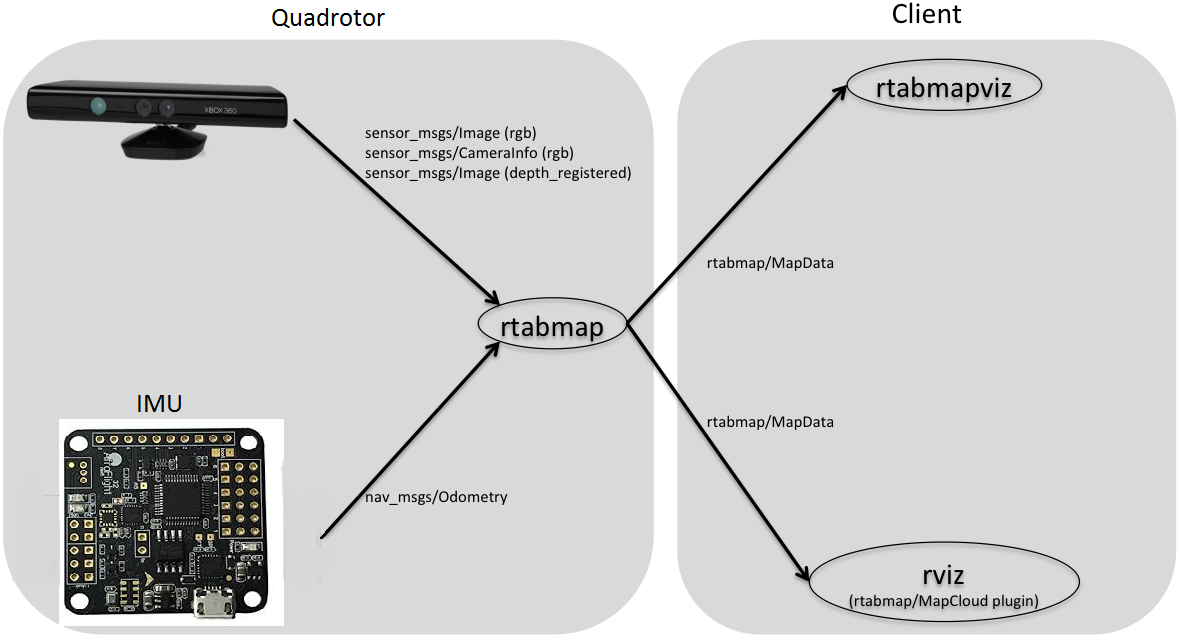
\includegraphics[width=2.5in]{setupC.png}
	\caption{Mapping with laptop}
	\label{fig_sim}
\end{figure}

\begin{figure}[ht]
	\centering
	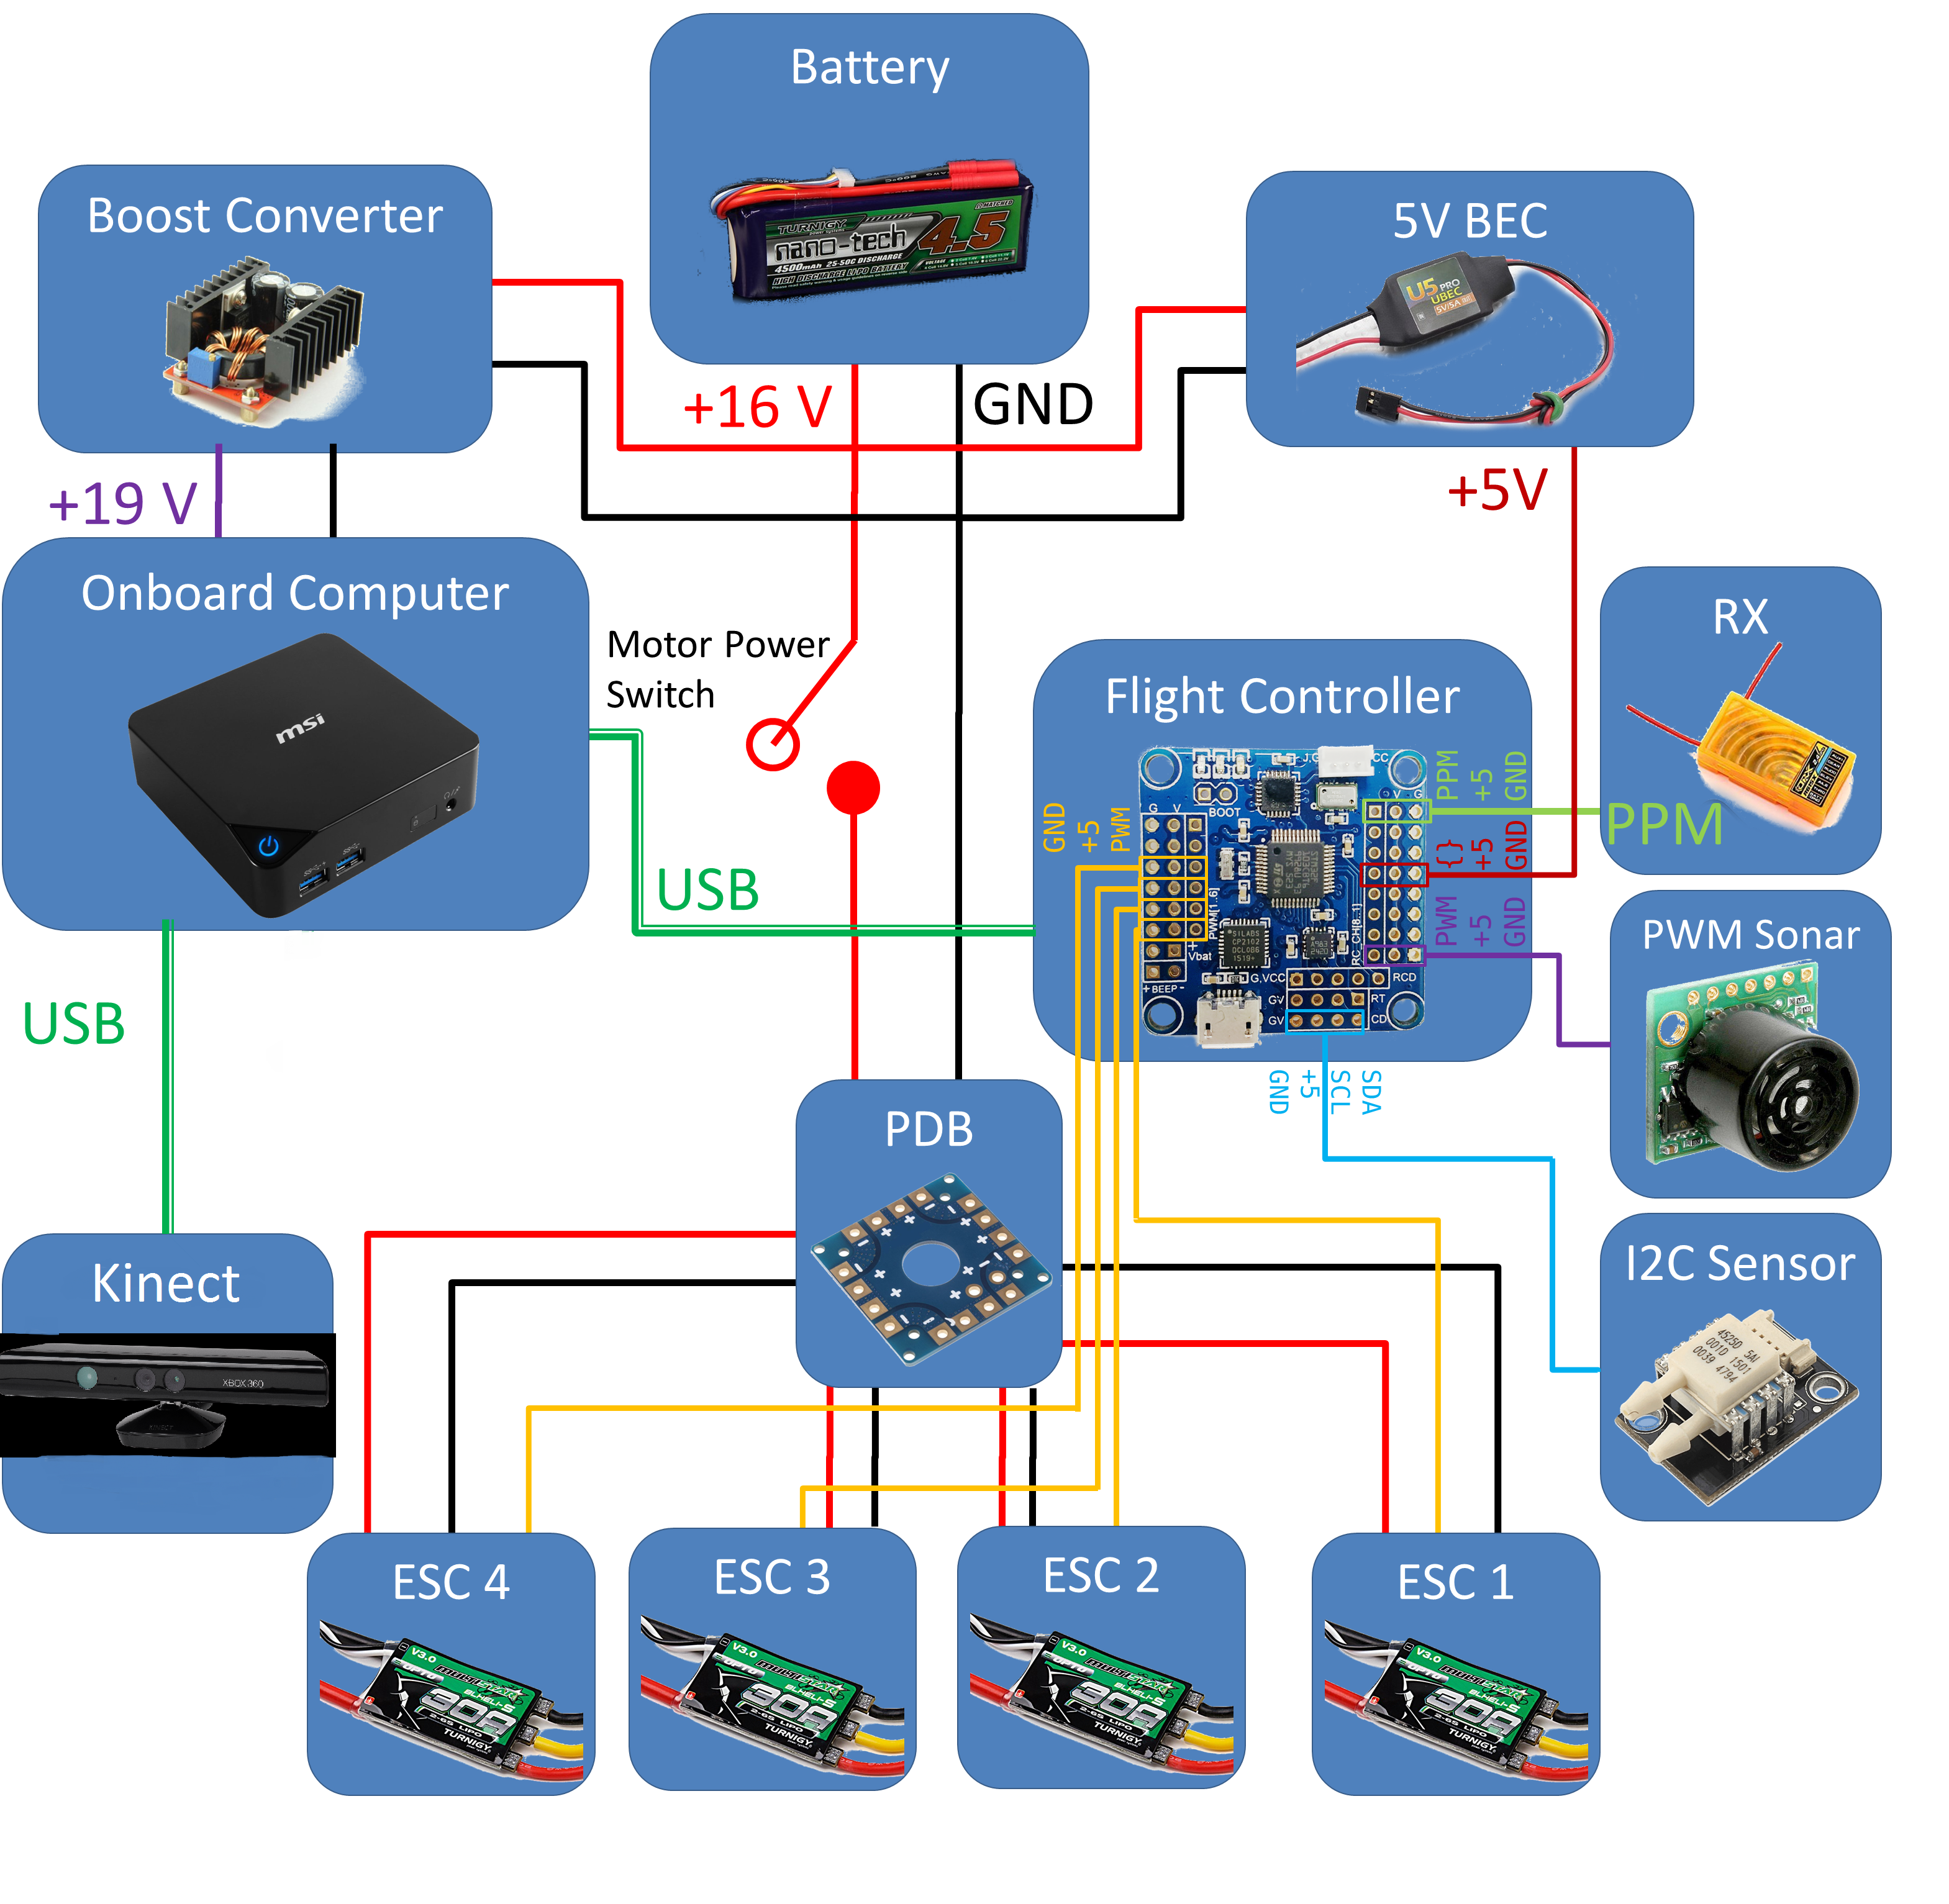
\includegraphics[width=2.5in]{Wiring_Diagram.png}
	\caption{Mapping with laptop}
	\label{fig_sim}
\end{figure}


\section{Results}
A frame rate of 20-25 fps is obtained when the Kinect is connected to the laptop, RTAB-Map does the mapping and RTAB-Mapviz/RViz visualizes the map. 

4-5 fps is obtained when the kinect is connected to the Raspberry Pi and mapping is done by it and the map is visualized on the laptop. The data stream from the Kinect has to be divided by two to allow the RPi to process it fast enough. RPi requires 80-100kbps bandwidth for transmitting the map over the network to the laptop.



\begin{figure}[ht]
\centering
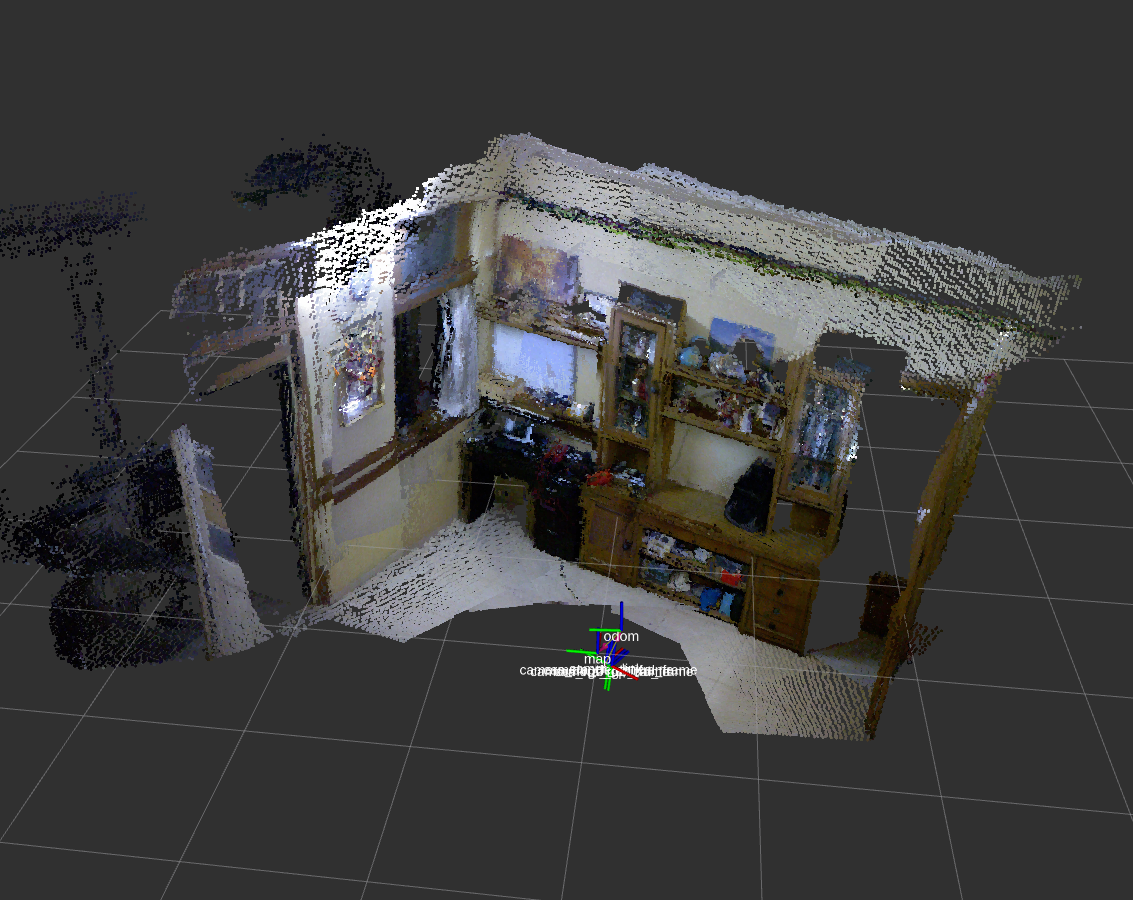
\includegraphics[width=2.5in]{1(1).png}
\caption{Mapping with laptop}
\label{fig_sim}
\end{figure}
 
\begin{figure}[ht]
	\centering
	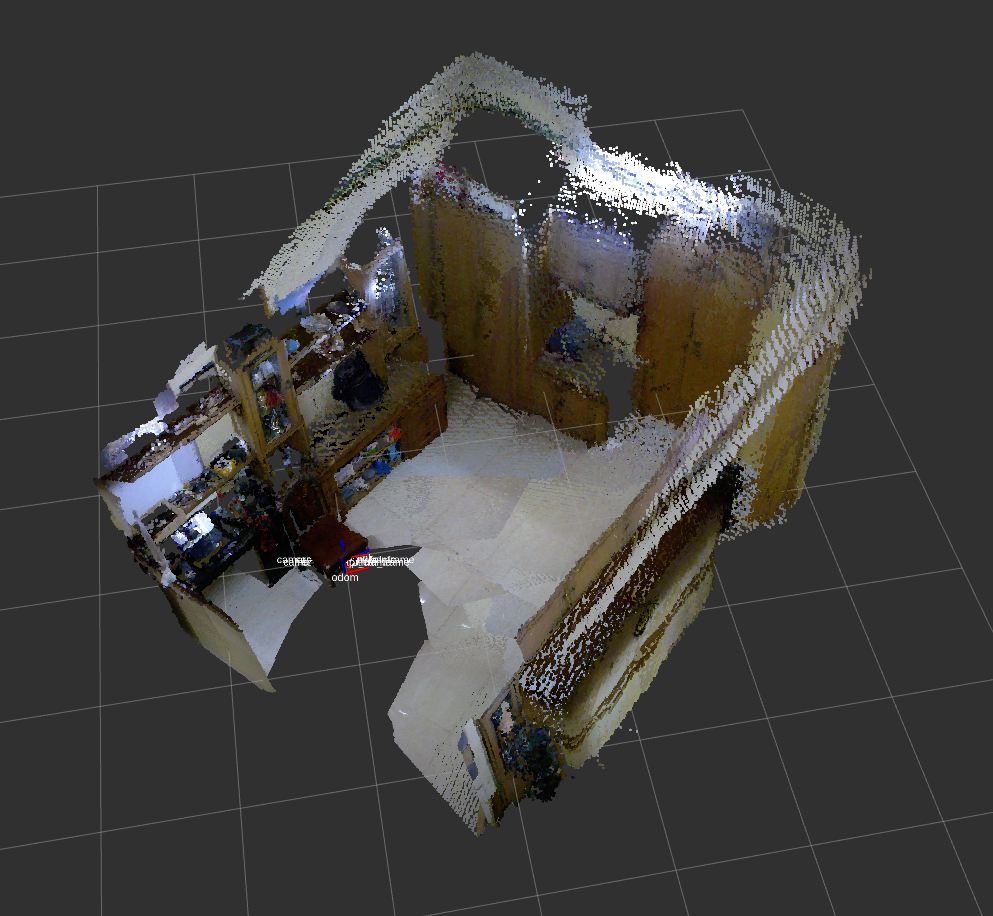
\includegraphics[width=2.5in]{1(2).png}
	\caption{Mapping with laptop}
	\label{fig_sim}
\end{figure}

\begin{figure}[ht]
	\centering
	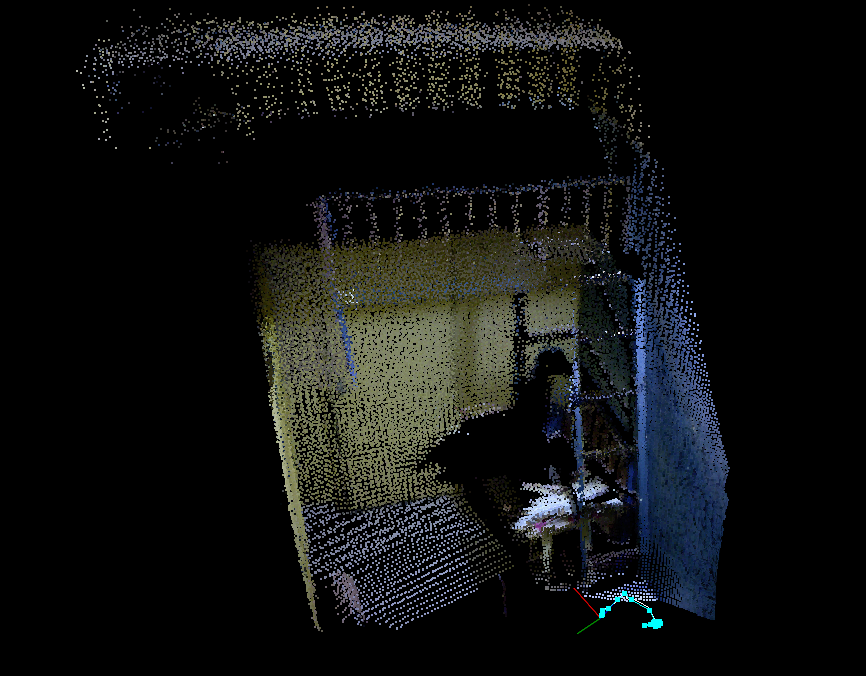
\includegraphics[width=2.5in]{2(1).png}
	\caption{Wireless Mapping with Raspberry Pi}
	\label{fig_sim}
\end{figure}

\begin{figure}[ht]
	\centering
	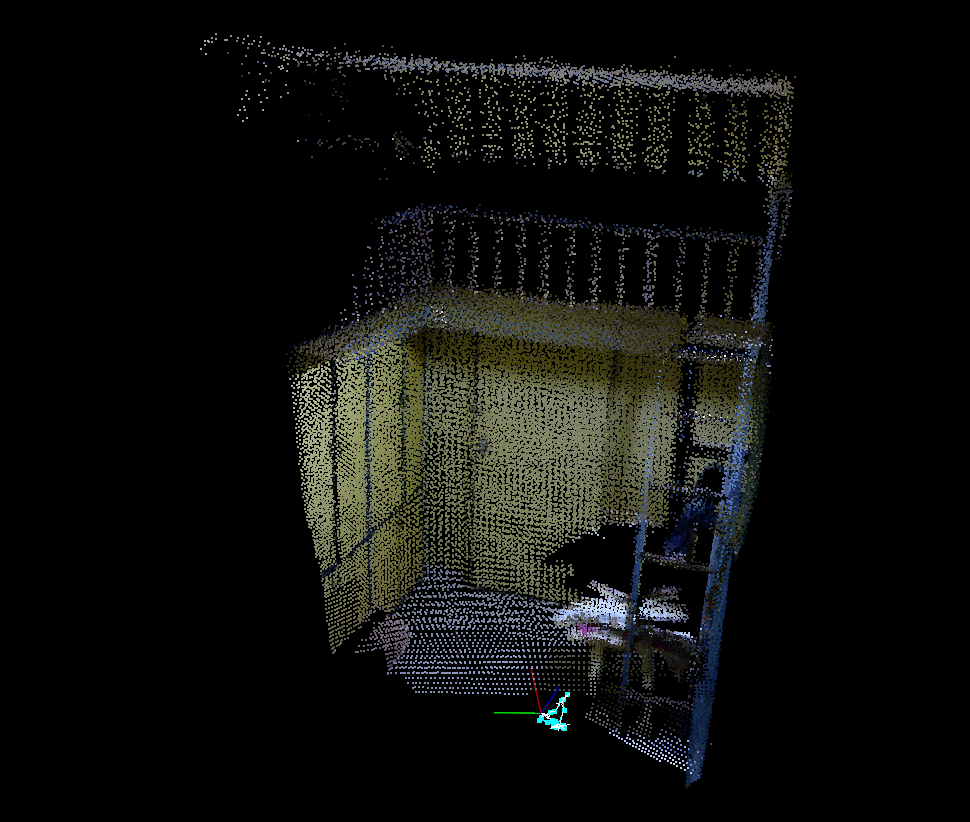
\includegraphics[width=2.5in]{2(2).png}
	\caption{Wireless Mapping with Raspberry Pi}
	\label{fig_sim}
\end{figure}

\section{Conclusion}
We were able to create a mobile system to generate a 3D map using the ROS framework on RPi and a Kinect sensor.
RPi provides a sufficient throughput for computing a 3D Map at 4-5 fps and transmit the same over a Wi-Fi.

This project enabled us to understand how the ROS framework works and how different packages integrate with each other.

\section*{Acknowledgment}

We would like to thank out mentor Kumar Khandagle for his support and guidance.

We would also like to thank our college Sardar Patel Institute of Technology for providing us with a platform for us to showcase our project.


% Can use something like this to put references on a page
% by themselves when using endfloat and the captionsoff option.
\ifCLASSOPTIONcaptionsoff
  \newpage
\fi



% trigger a \newpage just before the given reference
% number - used to balance the columns on the last page
% adjust value as needed - may need to be readjusted if
% the document is modified later
%\IEEEtriggeratref{8}
% The "triggered" command can be changed if desired:
%\IEEEtriggercmd{\enlargethispage{-5in}}

% references section

% can use a bibliography generated by BibTeX as a .bbl file
% BibTeX documentation can be easily obtained at:
% http://mirror.ctan.org/biblio/bibtex/contrib/doc/
% The IEEEtran BibTeX style support page is at:
% http://www.michaelshell.org/tex/ieeetran/bibtex/
%\bibliographystyle{IEEEtran}
% argument is your BibTeX string definitions and bibliography database(s)
%\bibliography{IEEEabrv,../bib/paper}
%
% <OR> manually copy in the resultant .bbl file
% set second argument of \begin to the number of references
% (used to reserve space for the reference number labels box)
\begin{thebibliography}{1}

\bibitem{RTAB-Map Paper 1}
M.~Labbé and F.~Michaud, \emph{"Appearance-Based Loop Closure Detection for Online Large-Scale and Long-Term Operation,"},
IEEE Transactions on Robotics, vol. 29, no. 3, pp. 734-745, 2013.

\bibitem{RTAB-Map Paper 2}
M.~Labbé and F.~Michaud, \emph{"Memory management for real-time appearance-based loop closure detection,"},
Proceedings of the IEEE/RSJ International Conference on Intelligent Robots and Systems, 2011, pp.1271–1276.

Memory management for real-time appearance-based loop closure detection,” in Proceedings of the IEEE/RSJ International Conference on Intelligent Robots and Systems.

\bibitem{RTAB-Map Paper 3}
M.~Labbé and F.~Michaud, \emph{"Online Global Loop Closure Detection for Large-Scale Multi-Session Graph-Based SLAM,"},
Proceedings of the IEEE/RSJ International Conference on Intelligent Robots and Systems, 2014.

\bibitem{RTAB-Map Paper 3}
Emarketer.com, 'Social Networking Reaches Nearly One in Four Around the World', 2014. [Online]. Available: 
http://introlab.github.io/rtabmap/. 
[Accessed: 31- Oct- 2017].

\end{thebibliography}

\end{document}


